As abondantly documented in the literature advection needs to be stabilised
as it otherwise showcases non-negligible under- and overshoots.
A standard approach is the Streamline Upwind Petrov Galerkin (SUPG) method.

\Literature \cite{brhu82}\cite{humm86}

%------------------------------
\subsubsection{Linear elements}

When using linear elements, its implementation is rather trivial, as shown in 
the DOUAR paper \cite{brtf08} or the FANTOM paper \cite{thie11}. 
The advection matrix is simply modified and computed as follows:
\[
({\bm K}_a^e)_{SUPG}
=
\int_{x_k}^{x_{k+1}}   ({\bm N}^\star)^T \rho C_p \vec\upnu \cdot {\bm B} dx  
\quad\quad
{\text with}
\quad\quad
{\bm N}^\star= {\bm N} + \tau \vec \upnu \cdot {\bm B}
\]
Note that we can also write 
\[
({\bm K}_a^e)_{SUPG}
=
\int_{x_k}^{x_{k+1}}   {\bm N}^T \rho C_p \vec\upnu \cdot {\bm B} dx  
+
\int_{x_k}^{x_{k+1}}  \tau (\vec \upnu \cdot {\bm B})^T   \rho C_p (\vec\upnu \cdot {\bm B}) dx  
\]
and we see that the SUPG method introduces and additional term that is akin to 
a diffusion term in the direction of the flow.
This can be seen by looking at the advection matrix a regular grid of 1D 
elements of size $h$:
\[
({\bm K}_a^e)_{SUPG}=
{\bm K}_a^e
+
\rho C_p
\frac{\tau u^2}{h}
\left(
\begin{array}{cc}
1 & -1 \\ \\
-1 & 1
\end{array}
\right)
\]
The additional matrix has the same structure as the 1D diffusion matrix matrix in \ref{sec:diff1D}.

The parameter $\tau$ is chosen as follows:
\begin{equation}
\tau=\gamma \frac{h}{\upnu} 
\label{tausupg}
\end{equation}
where $\gamma$ is a user chosen parameter (see Appendix A of \cite{thie11}). 

A typical test case for testing a advection scheme is the step advection benchmark (
see for instance \cite{dohu03}). At $t=0$, 
a field $T(x)$ is prescribed in a 1D domain of unit length. For $x\le 1/4$ we have $T(x)=1$ and 
$T(x)=0$ everywhere else as shown on the following figure:
\begin{center}
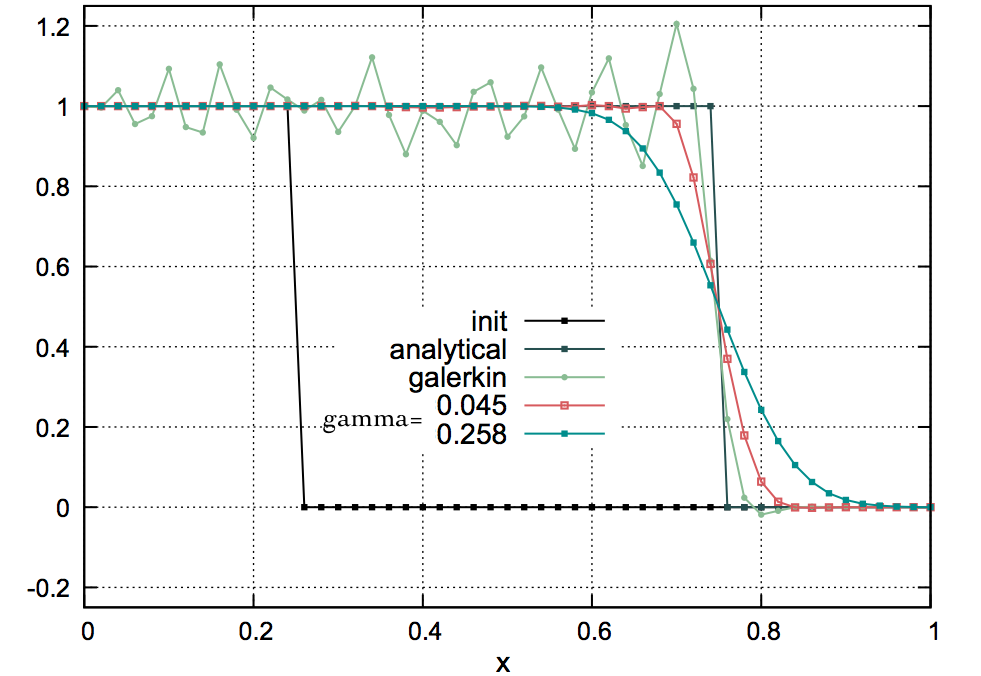
\includegraphics[width=8cm]{images/supg/fantom3}
\end{center}
The prescribed velocity is $\upnu=1$, 50 elements are used and 250 time steps are 
carried out with $\delta t=0.1h/\upnu=0.002$.
As discussed in \cite{thie11}, using Equation~\ref{tausupg}, 
one arrives to $\gamma=0.045$, which leads to a desired removal of the oscillations through a small
amount of numerical diffusion. Braun \cite{brau03} argues for a constant
$\gamma=1/\sqrt{15}=0.258$ (after \cite{hubr82}), which effect is also shown in the figure above. This 
value is arguably too large and introduces indesirable diffusion.








Another classic example of advection testing is a 2D problem where (for example) a cylinder, a Gaussian 
and a cone are prescribed and advected with a velocity field (see for instance \cite{dohu03}). 

\begin{center}
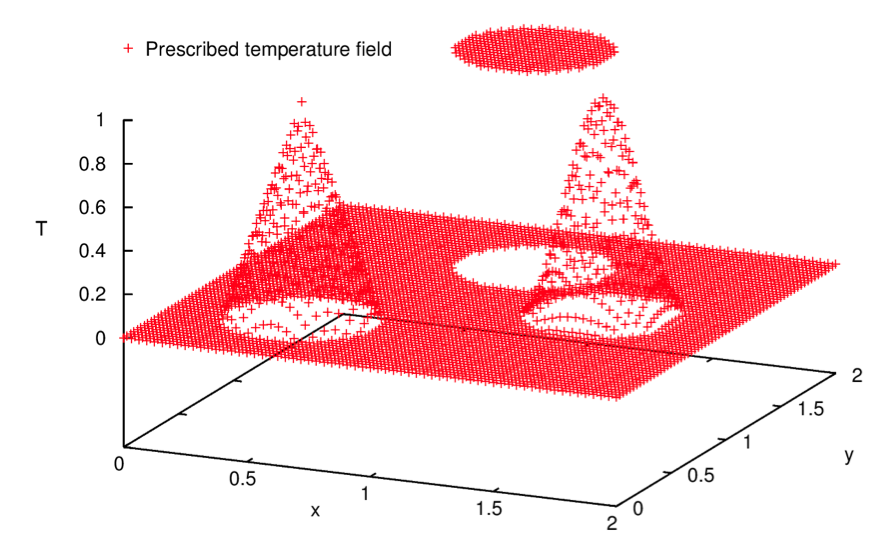
\includegraphics[width=0.45\textwidth]{images/supg/supg1}
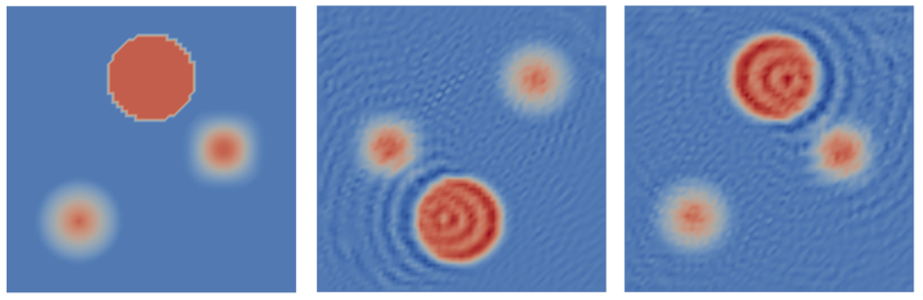
\includegraphics[width=0.45\textwidth]{images/supg/supg2}\\
{\captionfont After a $2\pi$ rotation and in the absence of stabilisation we see that the temperature field
showcases clearly visible ripples.}
\end{center}






\begin{remark}
Note that \aspect{} originally did not rely on the SUPG formulation to stabilise the 
advection(-diffusion) equations\cite{krhb12}. It instead relied on the Entropy Viscosity
formulation \cite{gupp11}.
It is only during the 6th Hackathon in May 2019 that the SUPG was introduced on the code.
Note that the \aspect{} implementation is based on the deal.II step 
63\footnote{\url{https://www.dealii.org/developer/doxygen/deal.II/step_63.html}}.
\end{remark}
